%%%%%%%%%%%%%%%%%%%%%%%%%%%%%%%%%%%%%%%%%%%%%%%%%%%%%%%%%%%%%%%%%%%%%%%%%%%%%%%%%%%%%%%%%%%%%%%%%%%%%%%%%%%%%%

\begin{exercise}{Potentiel mixte}{2}{Spé}
{Oxydoréduction, Courbes intensité potentiel}{bermu}

\begin{questions}
    \questioncours Potentiel mixte.
    \uplevel{Deux électrodes, l’une de fer et l’autre de zinc plongent dans une solution de chlorure de sodium (dont le seul rôle est d’assurer la conduction électrolytique). Elles sont court-circuitées.
    
    On observe un dégagement gazeux au niveau de l’électrode de fer et l’apparition d’un précipité blanc au niveau de l’électrode de zinc.}
    \question Interpréter ces observations à l’aide de courbes intensité-potentiel et évaluer le potentiel mixte de la solution.
\end{questions}

\paragraph{Données}

\begin{itemize}
    \item $E^\circ\qty\big(\mathrm{Fe^{2+}_{(aq)}/Fe_{(s)}}) = \SI{-0.44}{V}$
    \item $E^\circ\qty\big(\mathrm{Zn^{2+}_{(aq)}/Zn_{(s)}}) = \SI{-0.76}{V}$
    \item $\text{p}K_\text{s}(\mathrm{Zn(OH)_{2(s)}/Zr^{2+}_{(aq)}}) = 17.1$
    \item surtension du couple $\mathrm{H^+_{(aq)}/H_{2(g)}}$ sur le fer $\eta = \SI{-0.2}{V}$.
\end{itemize}

\end{exercise}

\begin{solution}

\begin{questions}
    \questioncours $j=0$ ne veut pas dire équilibre thermo !

    \begin{center}
        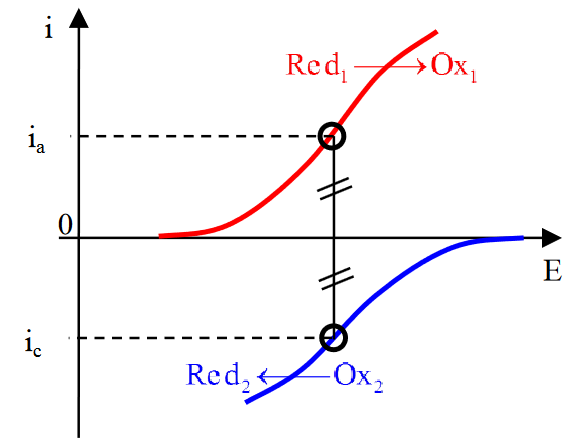
\includegraphics[scale=1.]{chimie/i-E/iE-cours3.png}
    \end{center}
    On observes spontanément un dégagement gazeux au niveau de l’électrode de fer et l’apparition d’un précipité blanc au niveau de l’électrode de zinc.
    \question Dégagement gazeux $=$ H$_2$. $\mathrm{2H^+_{(aq)} + 2 e^- \xrightarrow{Fe_{(s)}} H_{2(g)} }$.
    
    Précipité blanc $= \mathrm{Zn(OH)_{2(s)}}$. $\mathrm{Zn_{s(aq)} + 4 H_2O_{(\ell)} \xrightarrow{Zn_{(s)}} Zn(OH)_{2(s)} + 2H^+_{(aq)} + 2 e^- }$
    
~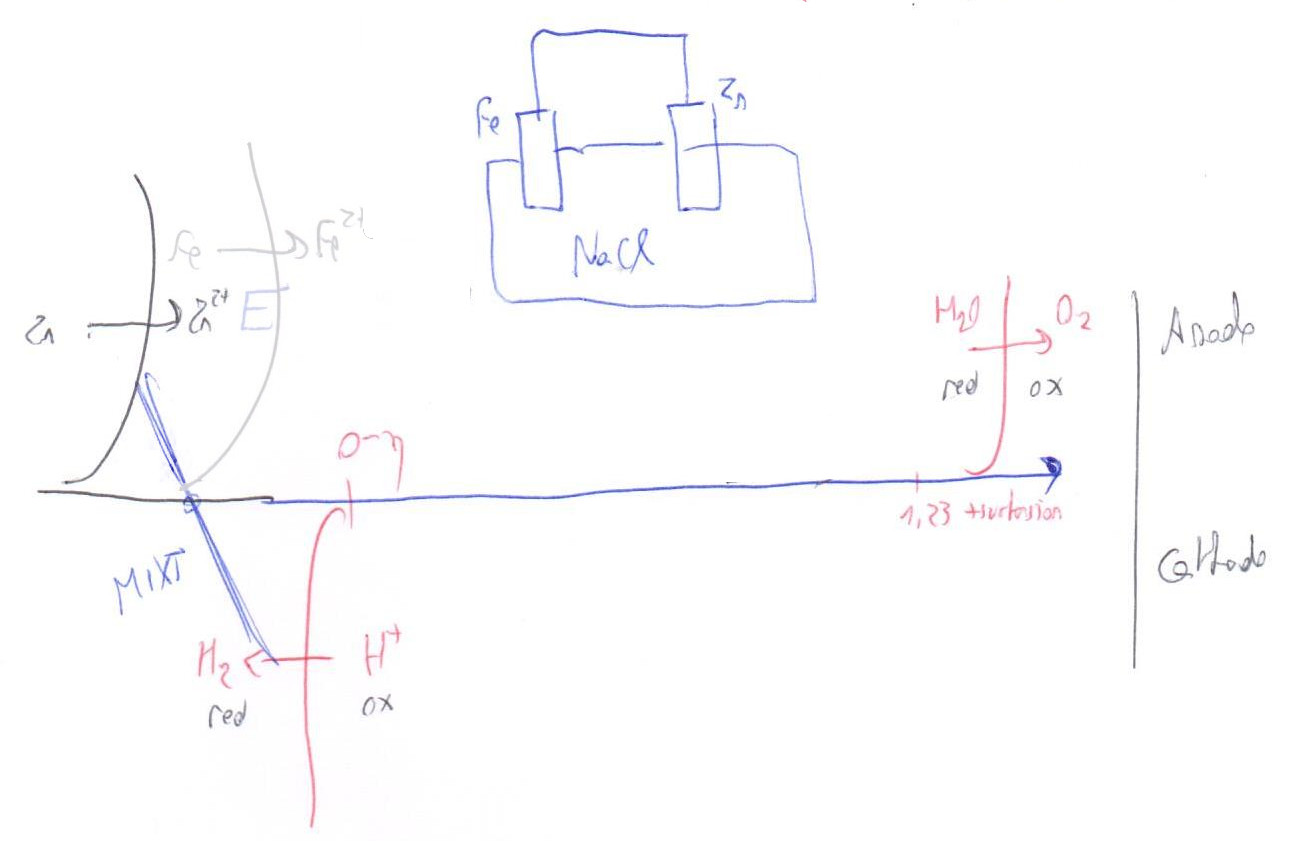
\includegraphics[width=\linewidth]{chimie/i-E/iE-corr2.jpg} 
\end{questions}

\end{solution}

%https://www.lycee-champollion.fr/IMG/pdf/td_no2_chimie_14-15.pdf